\chapter{提案手法}
\label{chap:提案手法}

本章では，ユーザーとAIが対等なパートナーとして音楽表現を共創するためのシステム構成，およびその具体的な処理手順について述べる．提案システムは，人間とAIが交互に演奏プランを提示し合うループ構造を基盤とし，言語モデルによる高度な意図解釈機能を組み込んでいる．

\section{システム概要}
\label{sec:システム概要}

提案システムの全体構成を図\ref{fig:proposed_system}に示す．
本システムは，既存の共創フレームワークであるICPLを拡張したものである．従来のICPLでは，ユーザーはAIが提示した候補についてランキング評価を行っていたが，本手法では自然言語によるフィードバック（コメント機能）を導入した．これにより，ユーザーは単なる「選択」だけでなく，「もう少し優しく」「テンポを揺らして」といった具体的な意図をエージェントに伝達することが可能となる．

\begin{figure}[h]
    \centering
    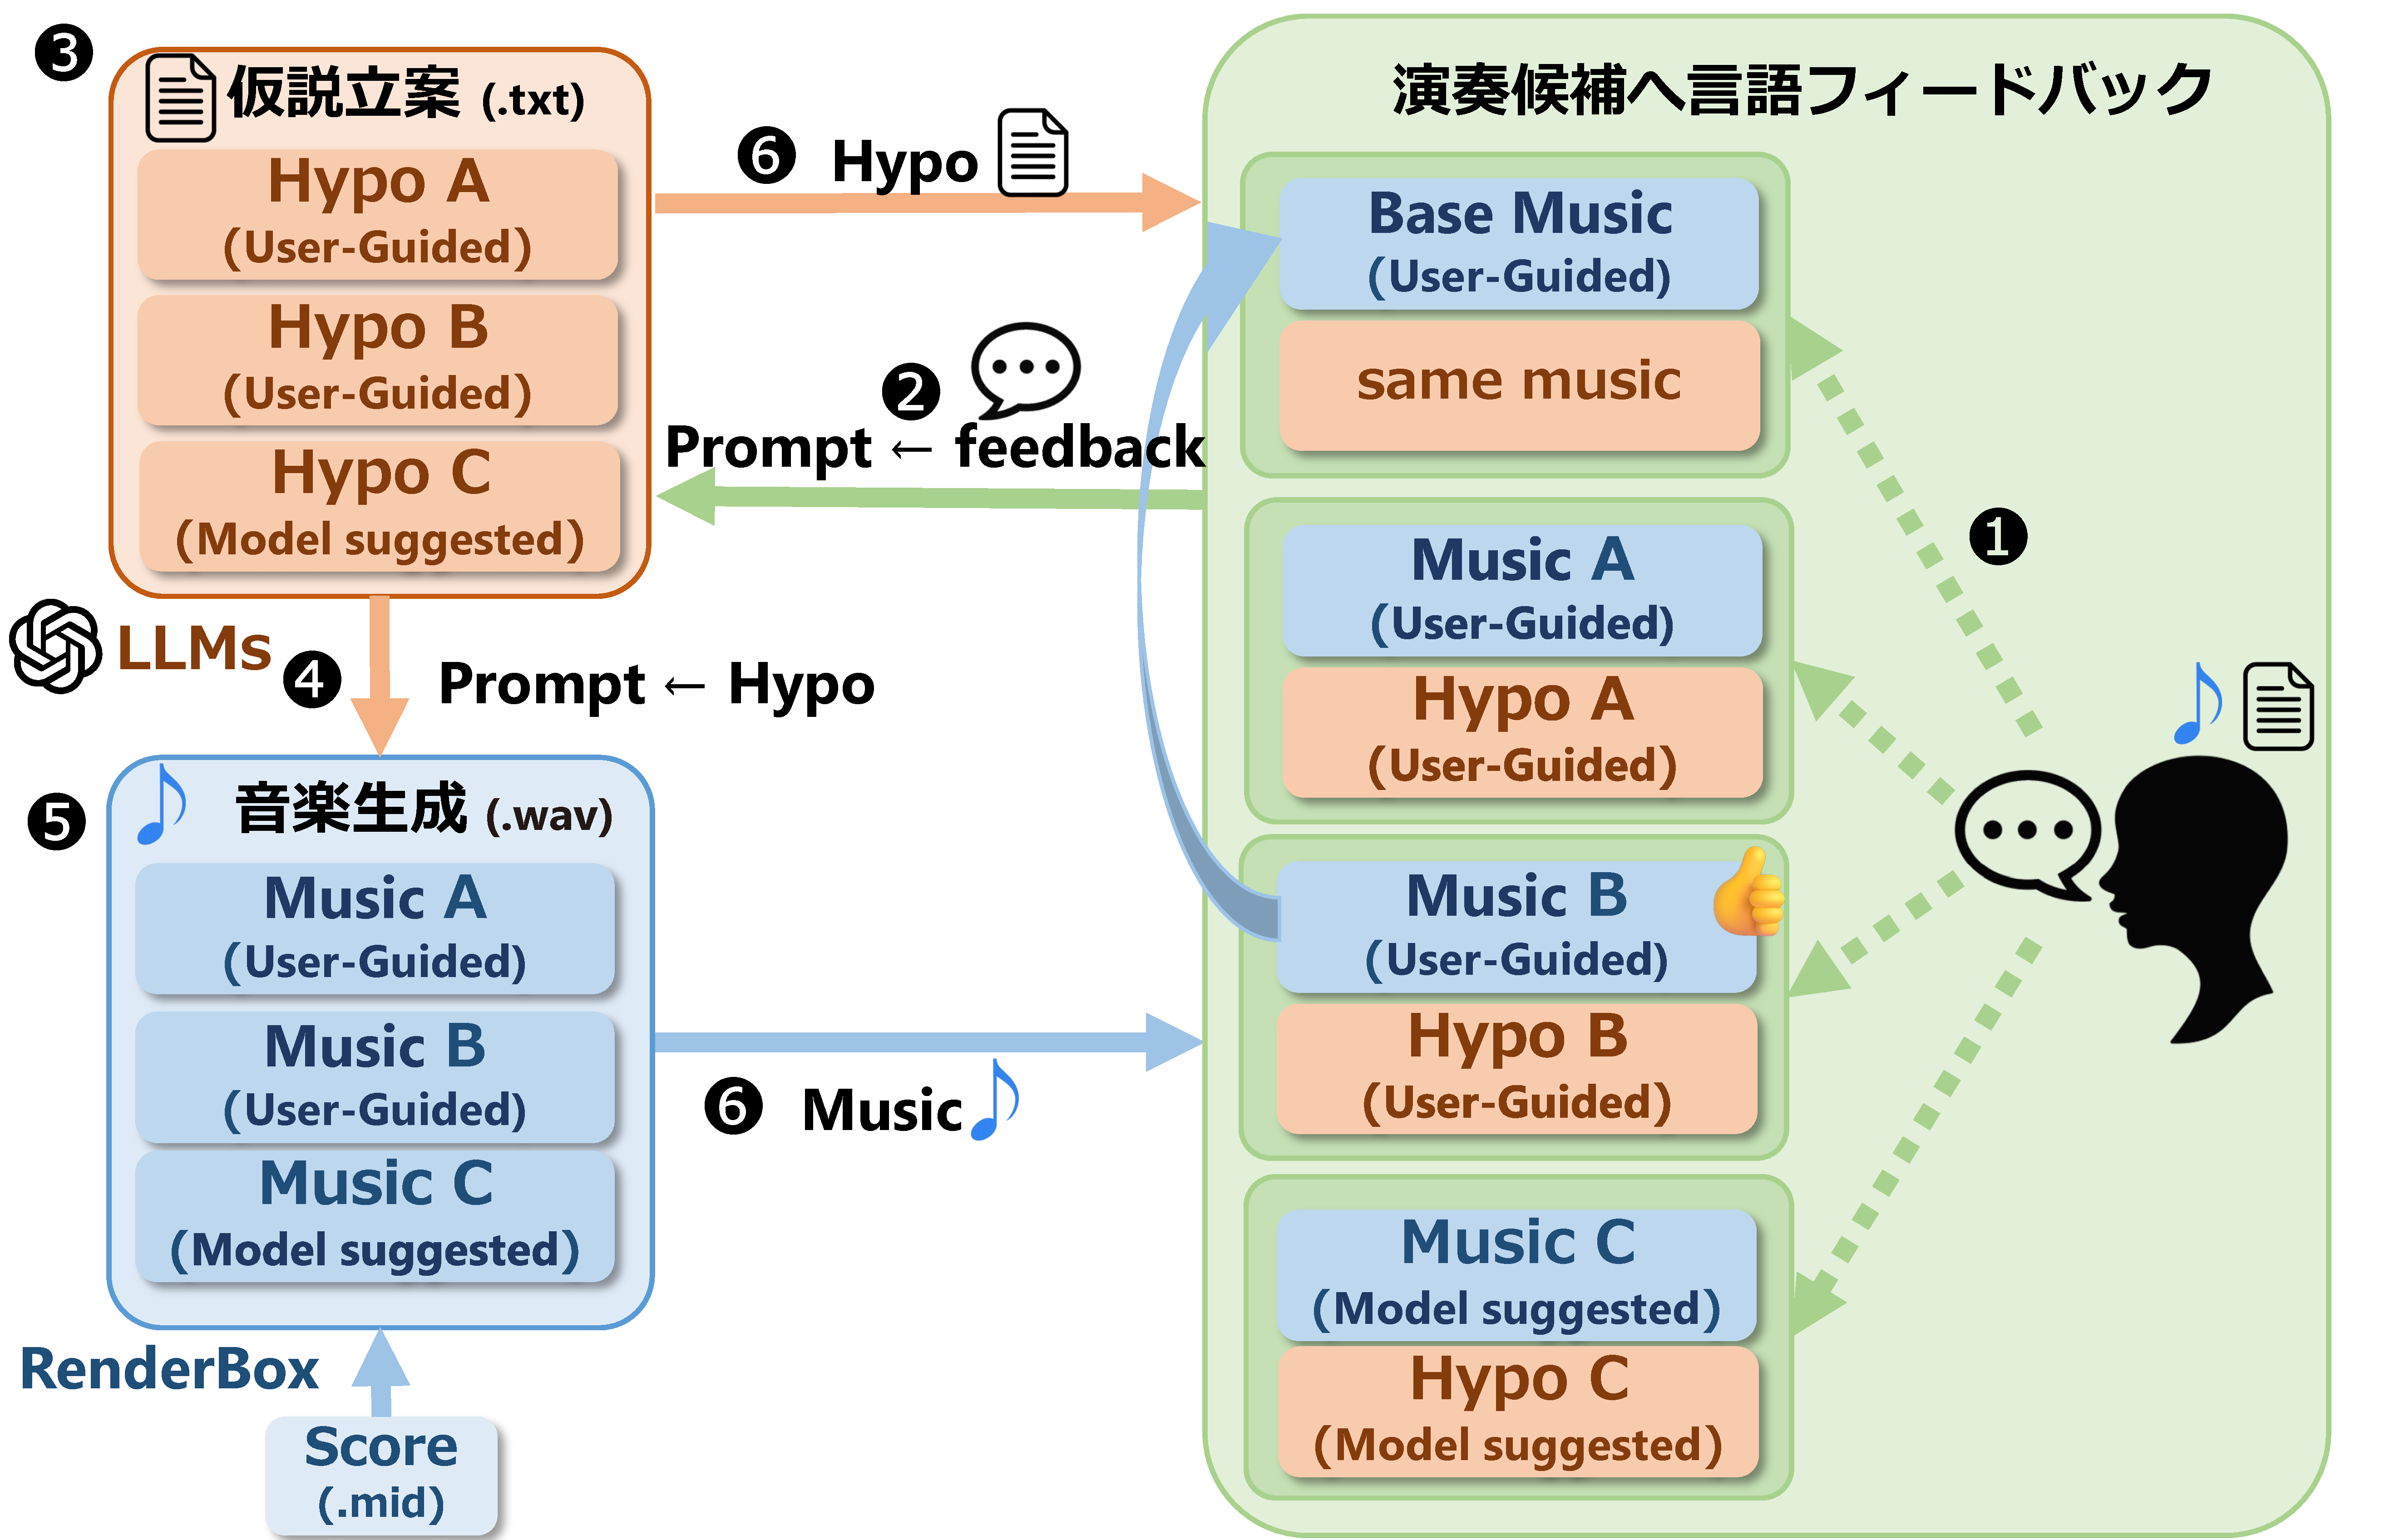
\includegraphics[width=1.0\linewidth]{figs/3/proposed_system.pdf}
    \caption{提案システム構成図}
    \label{fig:proposed_system}
\end{figure}

\section{対話システムとアルゴリズム}
\label{sec:対話システム}

本システムの核となる対話エージェント（Movot Agent）の推論エンジンには，OpenAIの \textbf{GPT-5} (reasoning\_effort=low) を採用した．このモデルは，ユーザーの抽象的な感性語を具体的な演奏パラメータ（強弱，速度，アーティキュレーションなど）へ変換する役割を担う．

システム全体の処理フローをアルゴリズム\ref{alg:overall}に，エージェント内部で行われる意図解釈と演奏生成の詳細プロセスをアルゴリズム\ref{alg:agent}に示す．

\begin{algorithm}
\caption{提案システムの全体処理アルゴリズム}
\label{alg:overall}
\begin{algorithmic}[1]
\Require Participant ID $ID$, Experiment Order $O \in \{Manual \to AI, AI \to Manual\}$

\State \textbf{Initialize:}
\State Load metadata $M$ (Title, Composer, Instrument) from database.
\State Analyze historical context $C_{hist}$ using LLM via \textit{analyze\_song.txt}.
\State Extract professional performance features $C_{perf}$ via \textit{MidiCaps} summary.
\State Generate initial synthesis $A_0$ with neutral prompt.

\State \textbf{Section 1 (Manual Prompting):}
\While{$step < Manual\_Target$}
    \State Receive user expression $E$ and speed index $S$.
    \State $P \gets$ Construct text prompt using $E$ and $SPEED\_TIERS[S]$.
    \State $D \gets$ Calculate duration based on $SPEED\_FACTORS[S]$.
    \State $A_{step} \gets$ AudioGeneration($P, MIDI, D$).
\EndWhile

\State \textbf{Section 2 (AI Co-Creation with Movot Agent):}
\State Initialize Agent with $C_{hist}$, $C_{perf}$, and $A_0$.
\While{$step < AI\_Target$}
    \State Execute \textbf{Algorithm 2} to generate three hypotheses.
    \State Present candidates $\{H_A, H_B, H_C\}$ to user.
    \State $Winner \gets$ User selection; Store feedback for next loop.
\EndWhile
\end{algorithmic}
\end{algorithm}

\begin{algorithm}
\caption{AIエージェントによる意図解釈と演奏生成のアルゴリズム}
\label{alg:agent}
\begin{algorithmic}[1]
\Require User Feedback $f_t$, Musical Context $M_1$ (Static), Interaction History $M_2$ (Dynamic)

\State \textbf{Holistic Feedback Analysis:}
\State $S_{curr} \gets$ Detect speed tag from the previous winner's prompt.
\If{$f_t$ requests speed change}
    \State Apply \textbf{AGGRESSIVE Speed Logic}: Shift speed category by 2 steps in $SPEED\_SCALE$.
\EndIf

\State \textbf{Hypothesis Generation (LLM Reasoning):}
\State \textbf{Strategy A (Direct):} Map $f_t$ strictly to musical articulation.
\State \textbf{Strategy B (Variation):} Propose alternative touch/style based on $f_t$.
\State \textbf{Strategy C (Contextual):} Blend $f_t$ with $C_{hist}$ and $C_{perf}$ from $M_1$.
\State \textbf{Constraint Check:} Ensure $H_A$ and $H_B$ use contrasting articulation (e.g., Legato vs. Rhythmic).

\State \textbf{Parallel Audio Synthesis:}
\For{each $H_i \in \{H_A, H_B, H_C\}$}
    \State $P_i \gets$ ``Expressive Performance, [Instrument], $H_i.keywords$''
    \State $D_i \gets$ Calculate duration for $H_i.speed\_tag$.
    \State $A_{i,t} \gets$ DiffusionModel($P_i, D_i, MIDI$).
\EndFor
\State \textbf{Output:} Reasoning logs and Audio candidates $\{A_A, A_B, A_C\}$.
\end{algorithmic}
\end{algorithm}



\begin{table}[htbp]
\centering
\caption{時系列順のLLMプロンプト構成とRoleの定義}
\label{tab:prompt_flow}
% \textwidth で「ページ幅いっぱい」を指定
% 最後の列を 'X' にすると、残りのスペースに合わせて自動改行されます
\begin{tabularx}{\textwidth}{l c l l} 
\hline
\textbf{フェーズ} & \textbf{Role} & \textbf{タイミング} & \textbf{提供される情報} \\ \hline
1. 楽曲分析 & System & 初期化時 & エージェントの役割 \\
 & & & 楽曲のタイトル \\
 & & & 作曲家名 \\ \hline
2. 状況設定 & System & 共創開始 & Movotの人格 \\
 & & & RenderBoxの能力 \\
 & & & プロ演奏のデータ \\ \hline
3. 対話ループ & User & 毎ループ実行 & 選択された演奏案 \\
 & & & フィードバック内容 \\
 & & & 過去の対話履歴 \\ \hline
4. 制約の適用 & User/System & 毎ループ実行 & 速度調整ルール \\
 & & & 提案間の差別化戦略 \\ \hline
\end{tabularx}
\end{table}



\section{UIの構築}
\label{sec:UIの構築}
PythonのGradioライブラリを用いて図？？のようなUIを作成した．